\documentclass{beamer}
\usepackage[utf8]{inputenc}
\usepackage[english]{babel}

\usepackage{url}
\usepackage{hyperref}
\usepackage{fancyvrb}
\usepackage{csquotes}
\usepackage{upquote}
\usepackage{../lib/diagrams}

\usepackage{amsmath}
\usepackage{amssymb}
\usepackage{amsthm}
\usepackage{tikz}
\usetikzlibrary{matrix}

\newcommand{\catx}[1]{\mathbb{#1}}
\newcommand{\catC}{\catx{C}}
\newcommand{\catD}{\catx{D}}

\newcommand{\opcat}[1]{{#1}^{\text{op}}}
\newcommand{\Sets}{\mathbf{Sets}}
\newcommand{\Cat}{\mathbf{Cat}}
\newcommand{\Hask}{\mathbf{Hask}}

%% @TODO: invent some kid of inline 'code' style for this
\newcommand{\firstArr}{\texttt{first}}

%% @TODO: pick a 'math' style for arrow operations
\newcommand{\arrM}{\text{arr}}
\newcommand{\firstM}{\text{first}}
%% >>>, <<< are \ggg and \lll

\DefineVerbatimEnvironment{code}{Verbatim}{fontsize=\small,commandchars=\\\{\},codes={\catcode`$=3\catcode`_=8}}

\hypersetup{
    colorlinks,
    linkcolor=black,
    citecolor=black,
    filecolor=black,
    urlcolor=black
}


\usetheme{default}
\usecolortheme{beaver}
\usefonttheme{structuresmallcapsserif}

\title{Cat Arrows}
\subtitle{What is a categorical semantics for arrows?}
\author[Vyšniauskas, Emerich]
{Ignas Vyšniauskas \and Johannes Emerich}
\institute{
  ILLC \\
  Universiteit van Amsterdam
}
\date{November 1, 2013}
\subject{Computer Science}

\begin{document}

\frame{\titlepage}

\begin{frame}
    \frametitle{This is a presentation on Arrows.}

\end{frame}

\begin{frame}
    \frametitle{What is a monad?}

    \begin{center}What is a monad?\end{center}

\end{frame}

\begin{frame}
    \frametitle{A monad is...}

    \center It is well known that a monad is a burrito.

    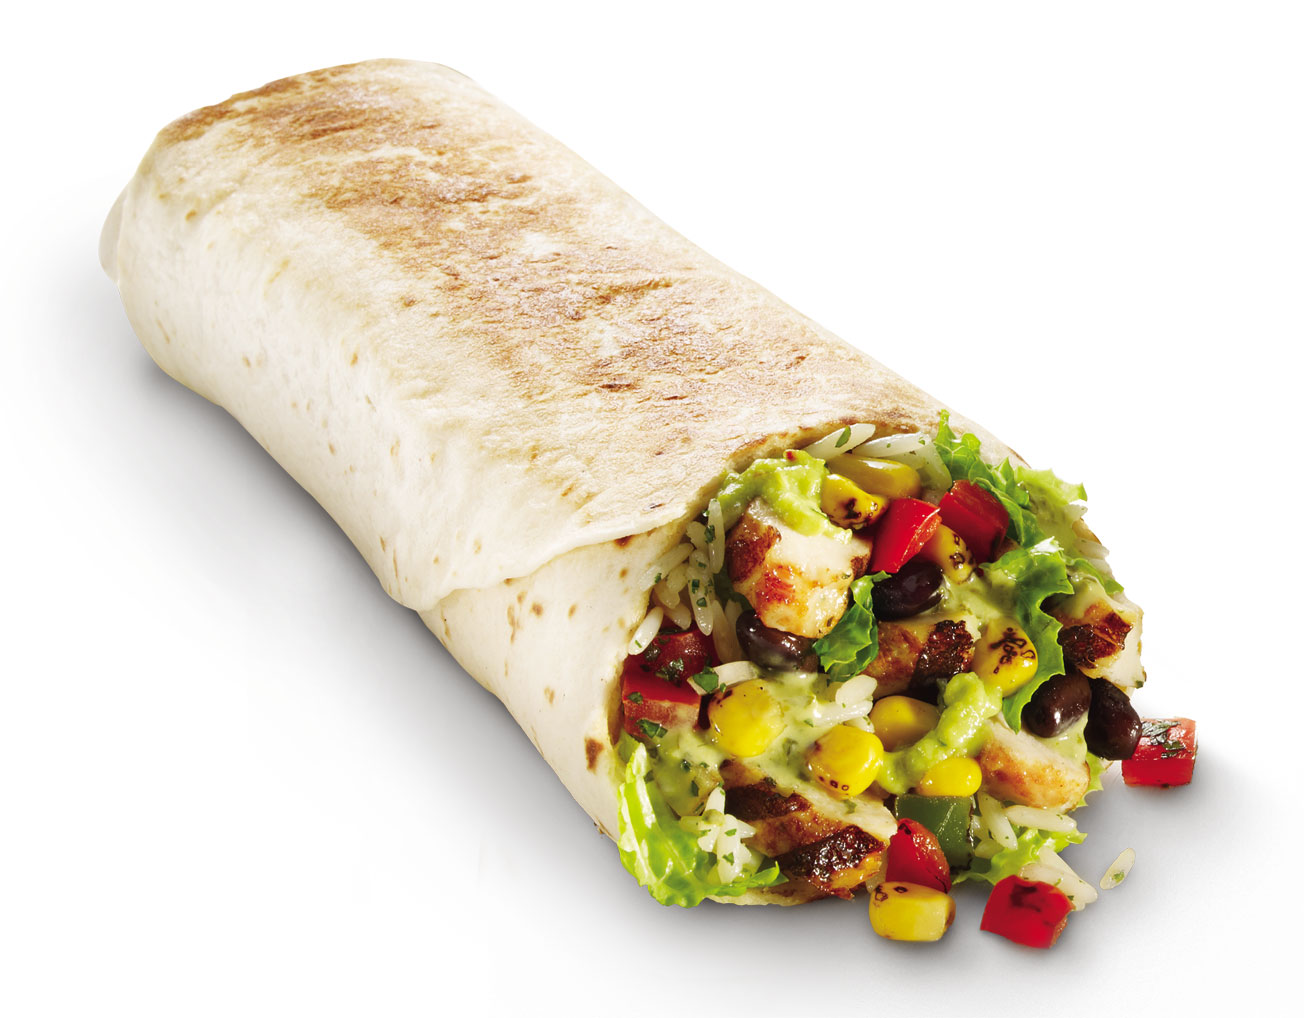
\includegraphics[width=0.8\textwidth]{img/burrito.jpg}

\end{frame}

\begin{frame}
    \frametitle{What is an arrow?}

    \begin{center}What is then an arrow?\end{center}

\end{frame}


\begin{frame}
    \frametitle{What is an arrow?}
    \center
    A taco, of course.
    \reflectbox{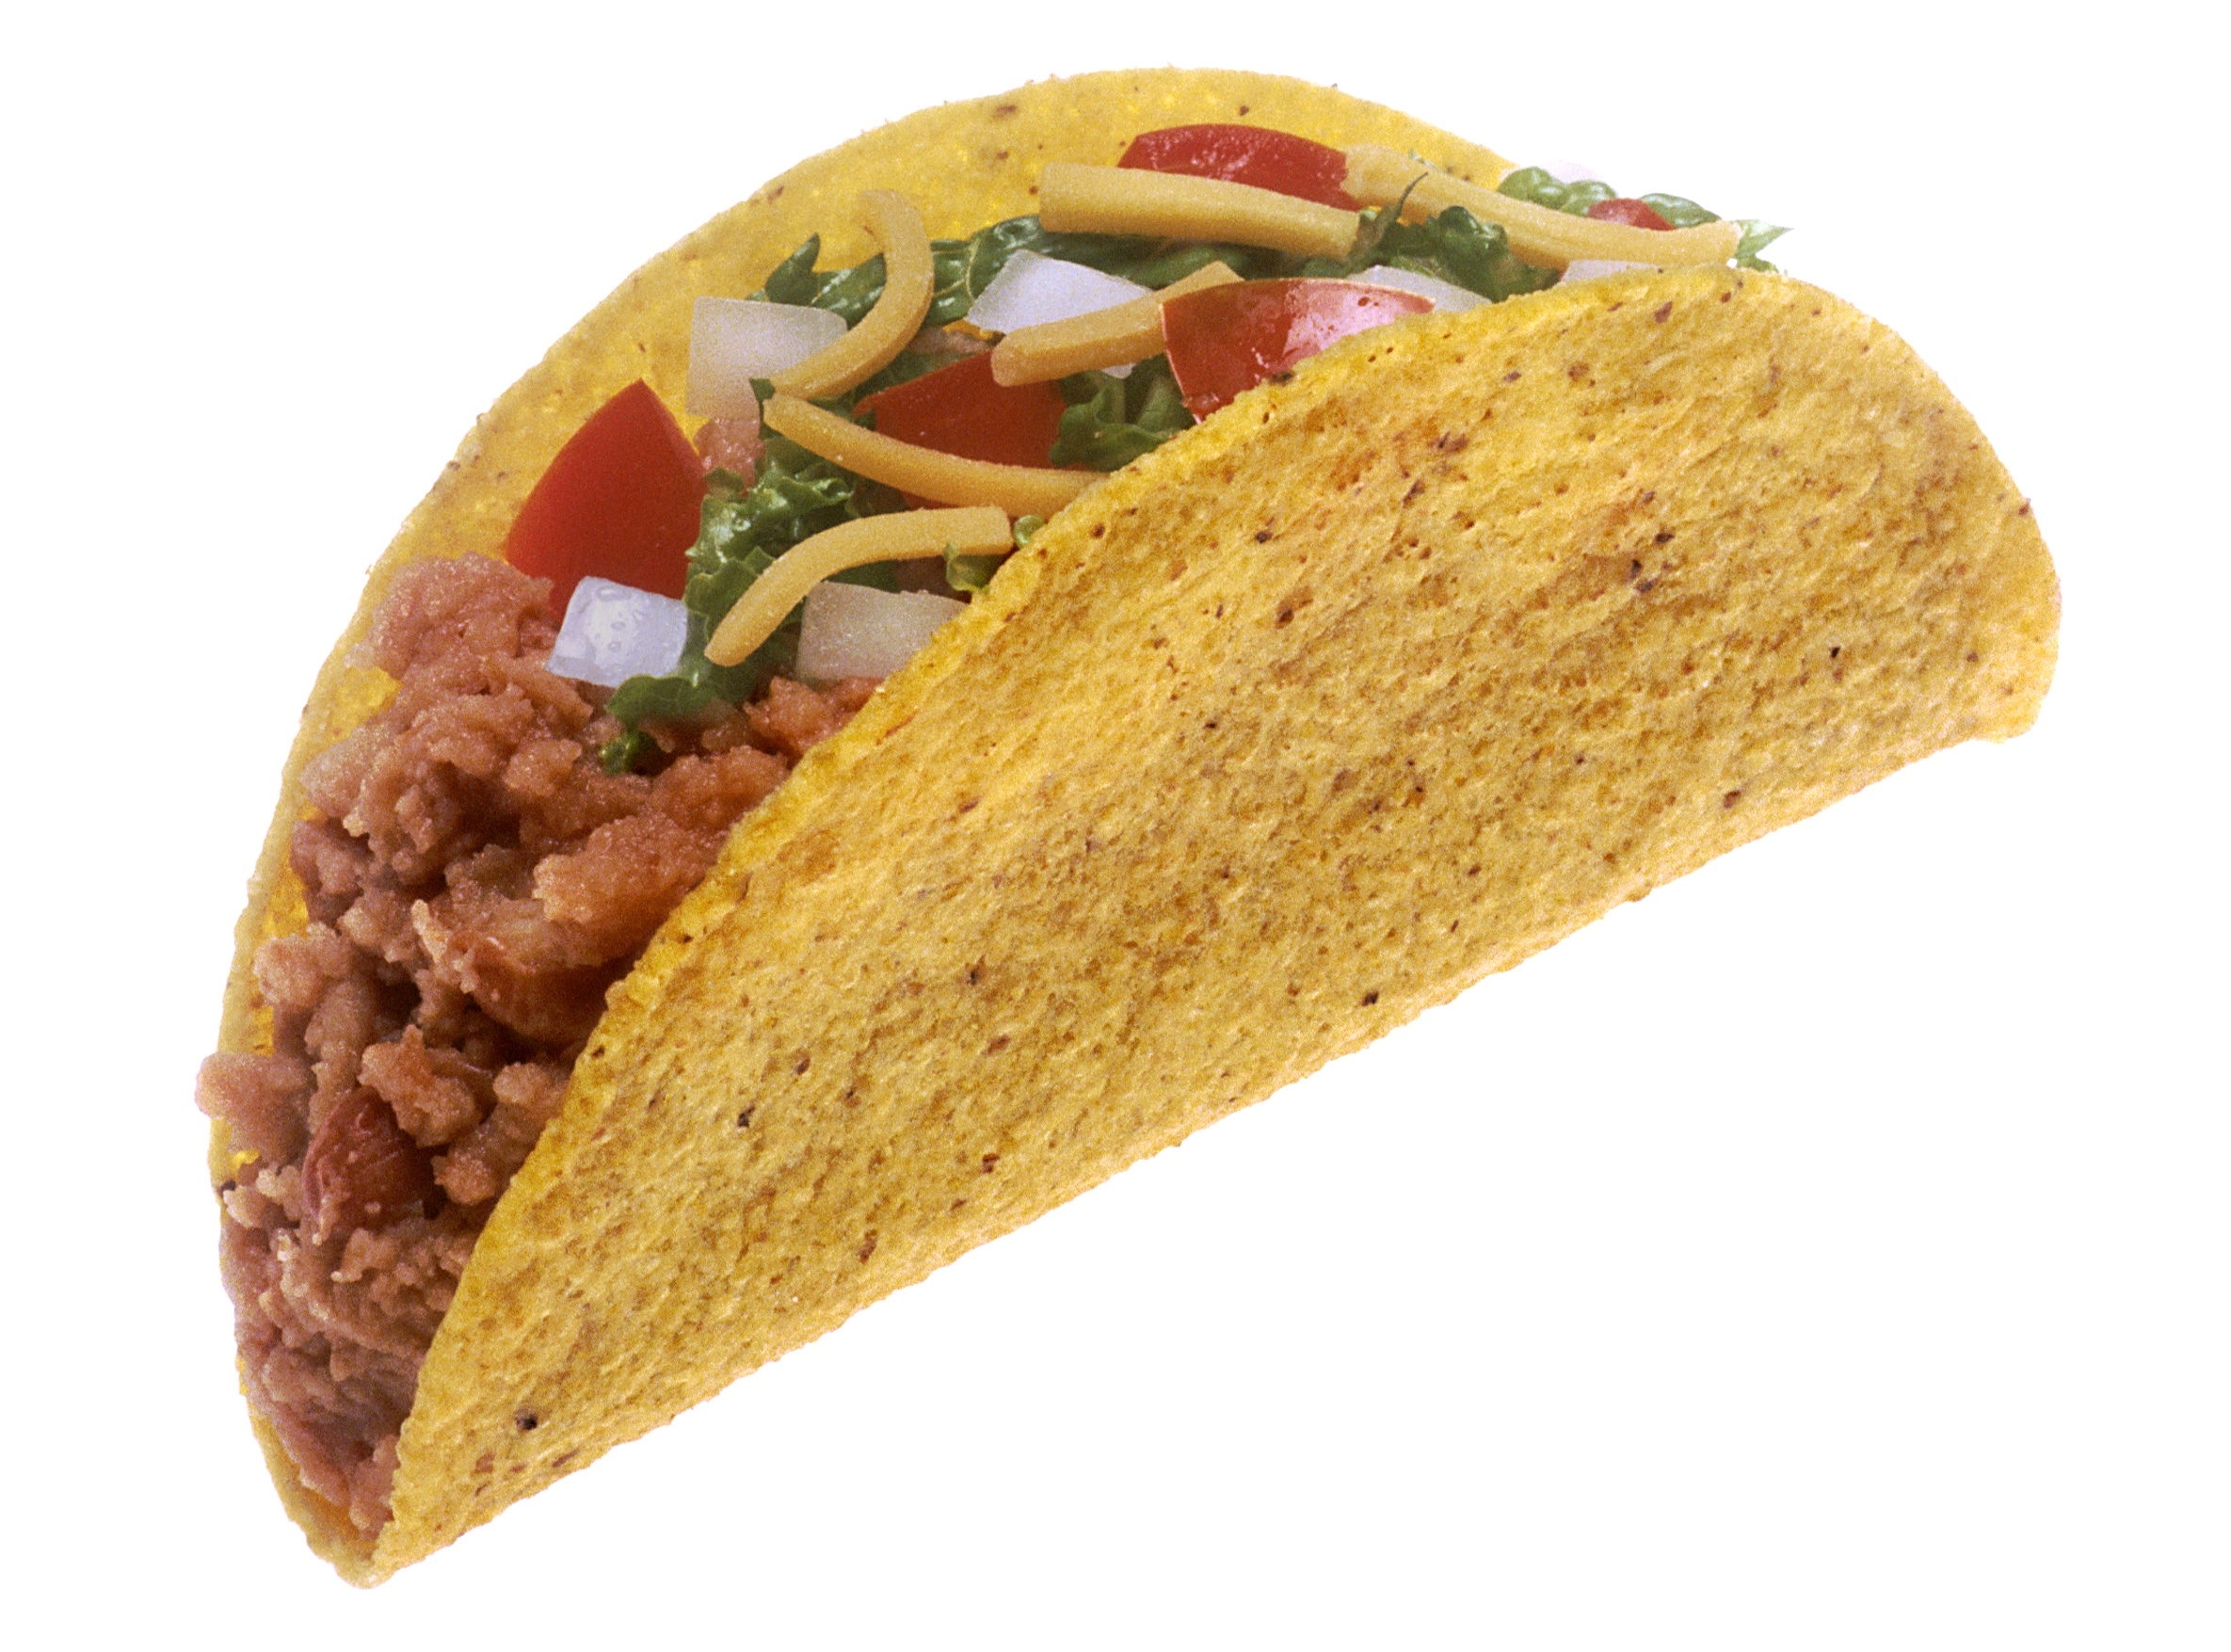
\includegraphics[width=0.8\textwidth]{img/taco.jpg}}

\end{frame}

\end{document}
